\section{Lösungsstrategie (DH)}
Um den Einstieg in die Lösung zu vereinfachen, ordnet Tabelle \ref{tab:QualitätszieleUndArchitekturansätze} den Qualitätszielen die Architekturansätze gegenüber. Abbildung \ref{fig:Loesungsansaetze_Ueberblick} verdeutlicht Aspekte der Systemarchitektur.
\begin{table}[htb]
	\centering
	\caption{Qualitätsziele und Architekturansätze}
	\label{tab:QualitätszieleUndArchitekturansätze}	
		\begin{tabular}{|l|l|}
		\hline
		Schnelle Abarbeitung der Aufträge & \textbullet{} Implementierung der Software in C++ \\
		 & \textbullet{} Vermeidung von unnötigen Arbeitswegen \\ 
		 & \textbullet{} Erläuterung der einzelnen Arbeitsschritte \\ 
		 & \textbullet{} Effiziente Implementierung der Backends \\ \hline
		Übersichtlichkeit & \textbullet{} Einhaltung von Usability-Normen \\ 
		 & \textbullet{} Einhaltung von Design-Tipps der Human Machine Interaction \\ \hline
		Verständlichkeit & \textbullet{} Einhaltung von Usability-Normen \\ 
		 & \textbullet{} Erläuterung der Dialoge \\
		 & \textbullet{} Verständliche Beschriftung der Eingabeelemente \\ \hline
		\end{tabular}
\end{table}
\begin{figure}[htb]
	\centering
		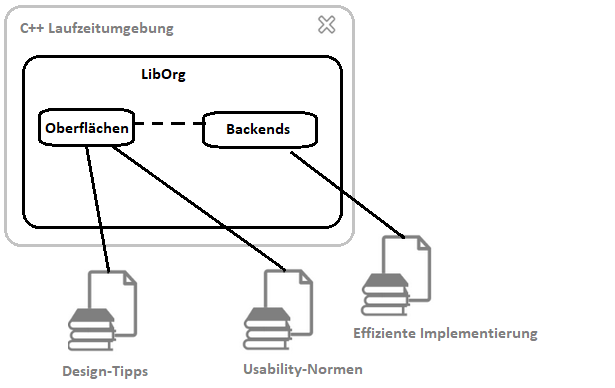
\includegraphics[width=0.60\textwidth]{figures/Loesungsansaetze_Ueberblick.png}
	\caption{Architekturaspekte Überblick}
	\label{fig:Loesungsansaetze_Ueberblick}
\end{figure}


\subsection{Aufbau von LibOrg}
LibOrg ist mittels C++ programmiert. Es ist wie folgt aufgeteilt:
\begin{itemize}
	\item db.dll: Schnittstelle zwischen der Anwendung und der Datenbank
	\item ExcelReader.dll: C++-Klasse zum Auslesen von Excel-Tabellen
	\item baseqt.dll: API, die Standardaufgaben übernimmt (z.B. Konfigurationen)
	\item Hauptanwendung
\end{itemize}
Durch die Aufteilung der Anwendung in die oben genannten Teile und die dynamische Verbindung zwischen ihnen ist es möglich, die Implementierung der entwickelten Bibliotheken (DLLs) zu erneuern, ohne dass die Hauptanwendung selber aktualisiert werden muss. Zudem wird der Wartungsaufwand der Anwendung erleichtert, da die Bibliotheken auch in anderen Projekten eingesetzt werden können (v.a. der ExcelReader und baseqt). Durch die Aufteilung der Anwendung in DLLs ist es ferner möglich, für jede DLL eigene Unit-Tests (falls gewünscht) zu entwickeln. Dies vereinfacht die Erstellung der Unit-Tests.\bigskip \\
Die Kommunikation der oben genannten Bestandteile der Software (DLLs und Hauptanwendung) erfolgt über Klassen. Bei der Implementierung der Klassen ist darauf geachtet worden, dass diese effizient und zugleich ohne lange Einarbeitungszeiten verständlich bzw. leserlich sind.\bigskip \\
Im Zentrum des Entwurfs der Strukturen liegt die Ausleihe/Rückgabe von Büchern: Für die Ausleihe wird ein Schüler-Objekt benötigt, ein Schüler kann mehrere oder keine Ausleihen haben. Außerdem ist eine Buch-Struktur notwendig, die ausgeliehen/zurückgeben wird. Die Datenstruktur für die Ausleihe enthält eine Struktur für die entsprechende Rückgabe. Das Zusammenspiel dieser Strukturen ist im Domänenmodell unter \ref{sec:domaenen} genauer verdeutlicht. Die Funktionsweise der Ausleihe/Rückgabe ist durch die Hauptanwendung definiert, wobei die Datenhaltung mit einer SQLite-Datenbank geregelt ist. Die Kommunikation findet über die Datenbank-API statt.


\subsection{Anbindungen}
LibOrg wird über eine grafische Benutzeroberfläche bzw. über grafische Benutzeroberflächen gesteuert. Die Interaktion mit dem Benutzer findet folglich über die Oberflächen statt, wobei der Benutzer durch einleitende Texte an die Verwendung der Software herangeführt wird.\bigskip \\
Durch den Einsatz von Qt arbeiten die Oberflächen mit dem Signal-Slot-Mechanismus, dieser entspricht dem Event-Ansatz. Beim Event-Ansatz wird von einem Element des GUI ein Event ausgelöst, das wiederum in einer Event-Loop abgearbeitet wird. Längere Arbeitsschritte müssen daher in eigenen Threads abgearbeitet werden, da anderenfalls die grafische Oberfläche nicht reagieren kann.\bigskip \\
An die Anwendung ist eine Datenbank (SQLite) angebunden. Die Software besitzt keine Schnittstellen nach außen, d.h. es können keine externen Funktionen in die Software eingebaut werden (die Software besitzt kein Plugin-System nach außen).
